\clearpage
\section{Fe}
\subsection{铁单质}
\subsubsection{物理性质}
\begin{itemize}
	\item 银白色固体,有金属性光泽;
	\item 容易被磁铁吸引;
	\item 地壳中居第四位;
\end{itemize}

\subsubsection{化学性质}
	铁元素性质活泼,有较强的还原性,主要化合价为+2价和+3价。
	\paragraph{与非金属单质反应} 
		\begin{itemize}
			\item $\ce{3Fe + 2O2 ->[\text{点燃}] Fe3O4}$
			\item $\ce{2Fe + 3Cl2 ->[\text{点燃}] FeCl3}$
			\item $\ce{Fe + S ->[\Delta] FeS}$
		\end{itemize}
	\paragraph{与水反应}
	铁在高温下与水蒸气反应
	$\ce{3Fe + 4H2O(g) ->[\text{高温}] Fe3O4 + 4H2}$
	\paragraph{与酸反应}
	铁遇到冷的浓硫酸或浓硝酸会钝化。
	\begin{itemize}
		\item 与非还原性酸:$\ce{Fe + 2H+ -> Fe^2+ + H2 ^}$
		\item 与还原性酸:$\ce{Fe + 4H+ + NO3- -> Fe^3+ + NO ^ + 2H2O}$
	\end{itemize}
	\paragraph{与盐溶液反应}
		\begin{itemize}
			\item 置换反应:$\ce{Fe + Cu^2+ -> Fe^2+ + Cu}$
			\item 与氯化铁溶液:$\ce{Fe + 2Fe^3+ -> 3Fe^2+}$ 
		\end{itemize}
		
\subsection{铁的氧化物}
\renewcommand\arraystretch{2}
\begin{center}
\begin{tabular}{|c|p{0.3\textwidth}<{\centering}|p{0.3\textwidth}<{\centering}|p{0.3\textwidth}<{\centering}|}
	\hline
	名称&氧化亚铁&氧化铁&四氧化三铁\\\hline
	俗称&-&铁红&磁性氧化铁\\\hline
	化学式&\ce{FeO}&\ce{Fe2O3}&\ce{Fe3O4}\\\hline
	化合价&+2&+3&+2、+3\\\hline
	物理性质&黑色粉末&\textcolor[rgb]{0.541,0.149,0.078}{红褐色}粉末&黑色晶体\\\hline
	与\ce{CO}反应&$\ce{FeO + CO ->[\Delta] Fe + CO2}$&$\ce{Fe2O3 + 3CO ->[\Delta] 2Fe + 3CO2}$&$\ce{Fe3O4 + 4CO ->[\Delta] 3Fe + 4CO2}$\\\hline
	与\ce{H2}反应&$\ce{FeO + H2 ->[\Delta] Fe + H2O}$&$\ce{Fe2O3 + 3H2 ->[\Delta] 2Fe + 3H2O}$&$\ce{Fe3O4 + 4H2 ->[\Delta] 3Fe + 4H2O}$\\\hline
	与酸反应&$\ce{FeO + 2H+ -> Fe^2+ + H2O}$&$\ce{Fe2O3 + 6H+ -> 2Fe^3+ + 3H2O}$&$\ce{Fe3O4 + 8H+ -> Fe^2+ + 2Fe^3+ + 4H2O}$\\\hline
\end{tabular}
\end{center}

\subsection{铁的水化物}
\subsubsection{比较\ce{Fe(OH)2}和\ce{Fe(OH)3}}
\begin{center}
\begin{tabular}{|c|c|c|}
	\hline
	名称&氢氧化亚铁&氢氧化铁\\\hline
	化学式&\ce{Fe(OH)2}&\ce{Fe(OH)3}\\\hline
	物理性质&白色固体&\textcolor[rgb]{0.541,0.149,0.078}{红褐色}固体\\\hline
	与酸反应&$\ce{Fe(OH)2 + 2H+ -> Fe^2+ + 2H2O}$&$\ce{Fe(OH)3 + 3H+ -> Fe^3+ + 3H2O}$\\\hline
	受热分解&$\ce{Fe(OH)2 ->[\Delta] FeO + H2O}$&$\ce{2Fe(OH)3 ->[\Delta] Fe2O3 + 3H2O}$\\\hline
	制备&$\ce{FeCl2 + 2NaOH -> Fe(OH)2 v + 2NaCl}$&$\ce{FeCl3 + 3NaOH -> Fe(OH)3 v + 3NaCl}$\\\hline
\end{tabular}
\end{center}
\subsubsection{\ce{Fe(OH)2}和\ce{Fe(OH)3}的转化}
\ce{Fe(OH)2}在空气中可以迅速被氧化成\ce{Fe(OH)3}。现象是由\textbf{白色絮状沉淀}迅速变成\textcolor[rgb]{0.231,0.301,0.219}{灰绿色},最后变成\textcolor[rgb]{0.541,0.149,0.078}{红褐色}。
$$\ce{4Fe(OH)2 + O2 + 2H2O -> 4Fe(OH)3}$$

\subsection{铁三角(铁、亚铁盐、铁盐)}
\begin{figure}[h]
\centering
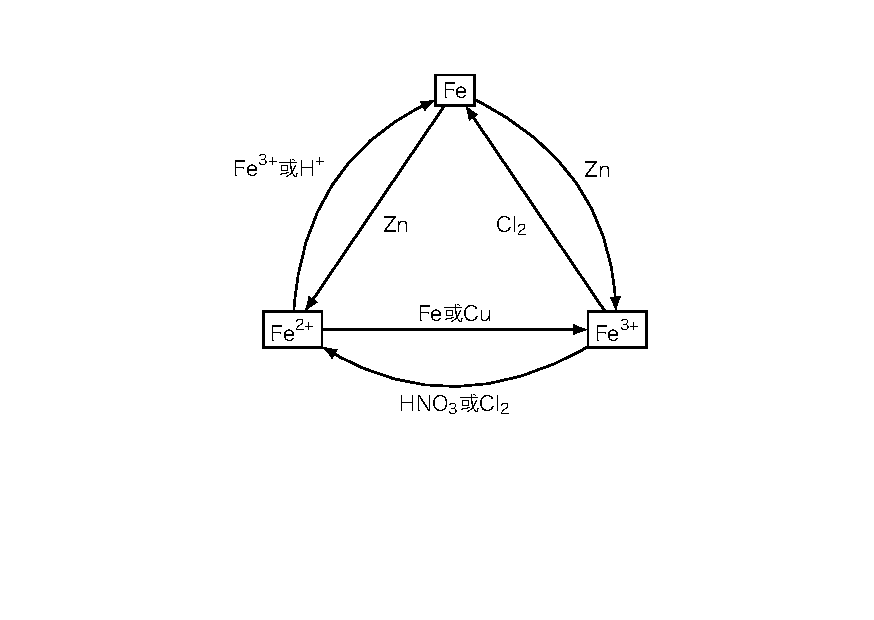
\includegraphics[scale=0.8]{res/Fe.pdf}
\end{figure}

\paragraph{亚铁盐}
含有\ce{Fe^2+}的溶液呈\textcolor[rgb]{0.625,0.8,0.7}{浅绿色},\ce{Fe^2+}既有氧化性,又有还原性。
\paragraph{铁盐}
含有\ce{Fe^3+}的溶液呈\textcolor[rgb]{0.835,0.611,0.247}{棕黄色}, \ce{Fe^3+}具有氧化性。含有\ce{Fe^3+}的盐溶液遇到\ce{KSCN}溶液时变成红色。
